\documentclass[conference]{IEEEtran}
\IEEEoverridecommandlockouts
\usepackage{iftex}
\usepackage{amsmath,amssymb}
\ifPDFTeX
  \usepackage[T1]{fontenc}
  \usepackage{mathptmx}
\else
  \usepackage{fontspec}
  \defaultfontfeatures{Ligatures=TeX}
  \setmainfont{texgyretermes}[Extension=.otf,UprightFont=*-regular,BoldFont=*-bold,ItalicFont=*-italic,BoldItalicFont=*-bolditalic]
  \setsansfont{texgyreheros}[Extension=.otf,UprightFont=*-regular,BoldFont=*-bold,ItalicFont=*-italic,BoldItalicFont=*-bolditalic]
  \setmonofont{texgyrecursor}[Extension=.otf,UprightFont=*-regular,BoldFont=*-bold,ItalicFont=*-italic,BoldItalicFont=*-bolditalic,Scale=MatchLowercase]
  \usepackage{unicode-math}
  \setmathfont{texgyretermes-math.otf}
\fi
\usepackage{cite}
\usepackage{graphicx}
\usepackage{array}
\usepackage{booktabs}
\usepackage{xcolor}
\usepackage{tikz}
\usetikzlibrary{arrows.meta,positioning,shapes.geometric,fit,calc}
\usepackage{url}
\usepackage[hidelinks]{hyperref}
% GENERATED by analysis/make_artifacts.py from analysis/outputs/results.json. Do not edit by hand.
\newcommand{\RFifty}{0.50}
\newcommand{\RFiftyHi}{0.79}
\newcommand{\RFiftyLo}{0.24}
\newcommand{\RSf}{0.81}
\newcommand{\RSfHi}{1.04}
\newcommand{\RSfLo}{0.56}
\newcommand{\RTen}{0.02}
\newcommand{\RTenHi}{0.15}
\newcommand{\RTenLo}{\ensuremath{-}0.13}
\newcommand{\RTf}{0.17}
\newcommand{\RTfHi}{0.40}
\newcommand{\RTfLo}{\ensuremath{-}0.06}
\newcommand{\acplHFifty}{105.45}
\newcommand{\acplHSf}{103.98}
\newcommand{\acplHTen}{107.77}
\newcommand{\acplHTf}{107.03}
\newcommand{\acplLaya}{107.86}
\newcommand{\acplMcts}{235.41}
\newcommand{\acplRandFifty}{105.36}
\newcommand{\acplRandSf}{104.22}
\newcommand{\acplRandTen}{107.35}
\newcommand{\acplRandTf}{106.66}
\newcommand{\acplSTwo}{103.06}
\newcommand{\acplSharp}{233}
\newcommand{\advFifty}{\ensuremath{-}0.09}
\newcommand{\advFiftyHi}{1.11}
\newcommand{\advFiftyLo}{\ensuremath{-}1.30}
\newcommand{\advSf}{0.24}
\newcommand{\advSfHi}{1.22}
\newcommand{\advSfLo}{\ensuremath{-}0.96}
\newcommand{\advTen}{\ensuremath{-}0.41}
\newcommand{\advTenHi}{0.17}
\newcommand{\advTenLo}{\ensuremath{-}0.96}
\newcommand{\advTf}{\ensuremath{-}0.37}
\newcommand{\advTfHi}{0.67}
\newcommand{\advTfLo}{\ensuremath{-}1.37}
\newcommand{\ancAlw}{6}
\newcommand{\ancHyb}{8}
\newcommand{\ancLaya}{11}
\newcommand{\ancMu}{1}
\newcommand{\ancThree}{12}
\newcommand{\aucBase}{0.591}
\newcommand{\aucBlunderLow}{0.46}
\newcommand{\aucChange}{0.69}
\newcommand{\aucConf}{0.607}
\newcommand{\aucConfHi}{0.627}
\newcommand{\aucConfLo}{0.585}
\newcommand{\aucDiff}{0.015}
\newcommand{\aucDiffHi}{0.038}
\newcommand{\aucDiffLo}{\ensuremath{-}0.008}
\newcommand{\aucHighForced}{0.83}
\newcommand{\aucImprove}{0.45}
\newcommand{\blunLaya}{17.3}
\newcommand{\blunMcts}{42.4}
\newcommand{\blunSTwo}{16.6}
\newcommand{\capFifty}{\ensuremath{-}0.47}
\newcommand{\capFiftyHi}{\ensuremath{-}0.20}
\newcommand{\capFiftyLo}{\ensuremath{-}0.74}
\newcommand{\capTwoHundred}{\ensuremath{-}1.59}
\newcommand{\capTwoHundredHi}{\ensuremath{-}0.70}
\newcommand{\capTwoHundredLo}{\ensuremath{-}2.51}
\newcommand{\chGainHigh}{110}
\newcommand{\chGainLow}{27}
\newcommand{\cnnEvals}{397}
\newcommand{\cohenDz}{0.072}
\newcommand{\confEnd}{0.18}
\newcommand{\confMed}{0.23}
\newcommand{\confMid}{0.16}
\newcommand{\confOpen}{0.11}
\newcommand{\confSharp}{0.44}
\newcommand{\constEnd}{0.0}
\newcommand{\constGainC}{1.8}
\newcommand{\constGainN}{5.1}
\newcommand{\constGainOpenC}{0.8}
\newcommand{\constGainOpenN}{0.6}
\newcommand{\constMid}{1.8}
\newcommand{\constN}{276}
\newcommand{\constOpen}{40.5}
\newcommand{\constPct}{9.2}
\newcommand{\constPlyMax}{35}
\newcommand{\costRatio}{3.2}
\newcommand{\dAbsHigh}{7.41}
\newcommand{\dAbsLow}{2.50}
\newcommand{\dAcpl}{\ensuremath{-}4.79}
\newcommand{\dAcplAbs}{4.79}
\newcommand{\dAcplHi}{\ensuremath{-}2.50}
\newcommand{\dAcplLo}{\ensuremath{-}7.41}
\newcommand{\dBigHi}{\ensuremath{-}2.49}
\newcommand{\dBigLo}{\ensuremath{-}7.29}
\newcommand{\dBlun}{\ensuremath{-}0.67}
\newcommand{\dBlunHi}{\ensuremath{-}0.20}
\newcommand{\dBlunLo}{\ensuremath{-}1.13}
\newcommand{\dClHi}{\ensuremath{-}2.44}
\newcommand{\dClLo}{\ensuremath{-}7.28}
\newcommand{\dGood}{1.03}
\newcommand{\dTop}{0.77}
\newcommand{\decChangeHigh}{2}
\newcommand{\decChangeLow}{20}
\newcommand{\decGainHigh}{8.3}
\newcommand{\decGainHighHi}{22.0}
\newcommand{\decGainHighLo}{0.1}
\newcommand{\depthLeaf}{6.5}
\newcommand{\depthMax}{20.9}
\newcommand{\eDAL}{\ensuremath{-}17}
\newcommand{\eDALHi}{9}
\newcommand{\eDALLo}{\ensuremath{-}42}
\newcommand{\eDHA}{\ensuremath{-}8}
\newcommand{\eDHAHi}{10}
\newcommand{\eDHALo}{\ensuremath{-}30}
\newcommand{\eDHL}{\ensuremath{-}25}
\newcommand{\eDHLHi}{\ensuremath{-}5}
\newcommand{\eDHLLo}{\ensuremath{-}49}
\newcommand{\eDLM}{170}
\newcommand{\eDLMHi}{216}
\newcommand{\eDLMLo}{126}
\newcommand{\eNoPriorHL}{\ensuremath{-}25}
\newcommand{\eceVal}{0.34}
\newcommand{\eloAlw}{887}
\newcommand{\eloAlwHi}{938}
\newcommand{\eloAlwLo}{821}
\newcommand{\eloHyb}{879}
\newcommand{\eloHybHi}{932}
\newcommand{\eloHybLo}{809}
\newcommand{\eloLaya}{904}
\newcommand{\eloLayaHi}{958}
\newcommand{\eloLayaLo}{832}
\newcommand{\eloMu}{734}
\newcommand{\eloMuHi}{783}
\newcommand{\eloMuLo}{668}
\newcommand{\fixedPct}{6.9}
\newcommand{\fracChanged}{8.2}
\newcommand{\fracEnd}{20}
\newcommand{\fracGainNeg}{3.5}
\newcommand{\fracGainPos}{4.0}
\newcommand{\fracGainZero}{92.5}
\newcommand{\fracPosGain}{4.0}
\newcommand{\fracSharp}{5.4}
\newcommand{\fullGain}{4.79}
\newcommand{\gainEnd}{11.0}
\newcommand{\gainEndHi}{18.1}
\newcommand{\gainEndLo}{4.7}
\newcommand{\gainMed}{14.6}
\newcommand{\gainMedHi}{28.2}
\newcommand{\gainMedLo}{3.1}
\newcommand{\gainMid}{4.1}
\newcommand{\gainMidHi}{7.3}
\newcommand{\gainMidLo}{1.1}
\newcommand{\gainOpen}{0.7}
\newcommand{\gainOpenHi}{3.5}
\newcommand{\gainOpenLo}{\ensuremath{-}1.5}
\newcommand{\gainPerSec}{4.6}
\newcommand{\gainSharp}{19.9}
\newcommand{\gainSharpHi}{44.7}
\newcommand{\gainSharpLo}{2.6}
\newcommand{\goodLaya}{48.6}
\newcommand{\goodMcts}{31.2}
\newcommand{\goodRateLaya}{48.6}
\newcommand{\goodSTwo}{49.7}
\newcommand{\hhDraws}{47}
\newcommand{\hhLosses}{3}
\newcommand{\hhP}{0.25}
\newcommand{\hhWins}{0}
\newcommand{\holmFifty}{1.00}
\newcommand{\holmTwentyFive}{1.00}
\newcommand{\hybSysShare}{74}
\newcommand{\impGten}{43}
\newcommand{\layaScored}{31.4}
\newcommand{\maxAdvHi}{1.22}
\newcommand{\maxAdvHiPct}{25}
\newcommand{\mdeFifty}{1.70}
\newcommand{\mdeSf}{1.55}
\newcommand{\mdeTen}{0.81}
\newcommand{\mdeTf}{1.46}
\newcommand{\meanConfAll}{0.15}
\newcommand{\medLaya}{28}
\newcommand{\medMcts}{121}
\newcommand{\medSTwo}{26}
\newcommand{\msLaya}{468}
\newcommand{\msLayaPart}{468}
\newcommand{\msMcts}{1042}
\newcommand{\msSTwo}{1499}
\newcommand{\msSearch}{1031}
\newcommand{\nBetter}{121}
\newcommand{\nChanged}{246}
\newcommand{\nChecks}{70}
\newcommand{\nChecksOk}{70}
\newcommand{\nDupGames}{196}
\newcommand{\nEnd}{600}
\newcommand{\nEqual}{21}
\newcommand{\nFixed}{36}
\newcommand{\nGamesA}{2{,}563}
\newcommand{\nIntro}{16}
\newcommand{\nLayaBlunder}{519}
\newcommand{\nMed}{292}
\newcommand{\nMid}{1800}
\newcommand{\nOpen}{600}
\newcommand{\nPos}{3{,}000}
\newcommand{\nPosGain}{121}
\newcommand{\nSharp}{161}
\newcommand{\nUniqSeq}{397}
\newcommand{\nWil}{225}
\newcommand{\nWorse}{104}
\newcommand{\oracleAcpl}{100.46}
\newcommand{\oracleCost}{571}
\newcommand{\oracleCostPct}{38}
\newcommand{\pBootFloor}{0.001}
\newcommand{\pFisherQ}{0.002}
\newcommand{\pFlip}{\ensuremath{2.5\times10^{-5}}}
\newcommand{\pHolmEnd}{0.001}
\newcommand{\pHolmMed}{0.064}
\newcommand{\pHolmMid}{0.060}
\newcommand{\pHolmOpen}{0.823}
\newcommand{\pHolmSharp}{0.097}
\newcommand{\pSign}{0.29}
\newcommand{\pT}{\ensuremath{8.7\times10^{-5}}}
\newcommand{\pWil}{0.003}
\newcommand{\posPerGameOne}{2{,}154}
\newcommand{\priorRatio}{63}
\newcommand{\puzAAlw}{4}
\newcommand{\puzAHyb}{1}
\newcommand{\puzAMu}{204}
\newcommand{\puzBAlw}{12}
\newcommand{\puzBHyb}{3}
\newcommand{\puzBMu}{99}
\newcommand{\puzDAlw}{0.8}
\newcommand{\puzDAlwHi}{1.6}
\newcommand{\puzDAlwLo}{0.1}
\newcommand{\puzDHyb}{0.2}
\newcommand{\puzDHybHi}{0.6}
\newcommand{\puzDHybLo}{\ensuremath{-}0.2}
\newcommand{\puzDMu}{\ensuremath{-}10.5}
\newcommand{\puzDMuHi}{\ensuremath{-}7.0}
\newcommand{\puzDMuLo}{\ensuremath{-}13.7}
\newcommand{\puzMaxBucket}{2.0}
\newcommand{\puzPAlw}{0.077}
\newcommand{\puzPHyb}{0.625}
\newcommand{\puzPMu}{0.000}
\newcommand{\puzPoolAlw}{44.6}
\newcommand{\puzPoolHyb}{44.0}
\newcommand{\puzPoolLaya}{43.8}
\newcommand{\puzPoolMu}{33.3}
\newcommand{\qDiff}{\ensuremath{-}5.9}
\newcommand{\qDiffHi}{\ensuremath{-}2.0}
\newcommand{\qDiffLo}{\ensuremath{-}9.3}
\newcommand{\qFour}{18.5}
\newcommand{\qOne}{12.7}
\newcommand{\qRatio}{0.68}
\newcommand{\qRatioHi}{0.88}
\newcommand{\qRatioLo}{0.54}
\newcommand{\randRFifty}{0.52}
\newcommand{\randSd}{0.61}
\newcommand{\rateFifty}{52.1}
\newcommand{\rateSf}{75.9}
\newcommand{\rateTen}{10.5}
\newcommand{\rateTf}{25.0}
\newcommand{\rhoChanged}{0.16}
\newcommand{\rhoConfCpl}{\ensuremath{-}0.18}
\newcommand{\rhoForced}{0.30}
\newcommand{\rhoGain}{0.01}
\newcommand{\rhoGainHi}{0.05}
\newcommand{\rhoGainLo}{\ensuremath{-}0.03}
\newcommand{\rrDraw}{75}
\newcommand{\rrN}{300}
\newcommand{\rrThree}{223}
\newcommand{\rrThreeHi}{79}
\newcommand{\rrThreeLo}{69}
\newcommand{\rrThreePct}{74.3}
\newcommand{\saAll}{3.8}
\newcommand{\saEnd}{0.0}
\newcommand{\saMid}{0.4}
\newcommand{\saN}{150}
\newcommand{\saOpen}{10.9}
\newcommand{\saSame}{100}
\newcommand{\sdDiff}{66.8}
\newcommand{\searchOverLaya}{2.2}
\newcommand{\shaNetHead}{924777b1}
\newcommand{\shaNetTail}{316e1b28}
\newcommand{\shareEnd}{46}
\newcommand{\shareFifty}{52.3}
\newcommand{\shareSf}{76.2}
\newcommand{\shareSharp}{22}
\newcommand{\shareTen}{10.5}
\newcommand{\shareTf}{25.2}
\newcommand{\sumNeg}{7808}
\newcommand{\sumPos}{22179}
\newcommand{\swBase}{136.2}
\newcommand{\swLaya}{108.4}
\newcommand{\swTone}{105.5}
\newcommand{\swTthree}{136.2}
\newcommand{\swTz}{97.5}
\newcommand{\tStat}{3.93}
\newcommand{\tauFifty}{0.0841}
\newcommand{\tauSeventyFive}{0.1713}
\newcommand{\tauTen}{0.0484}
\newcommand{\tauTwentyFive}{0.0576}
\newcommand{\topLaya}{26.2}
\newcommand{\topMcts}{17.7}
\newcommand{\topSTwo}{27.0}
\newcommand{\tostFifty}{1.10}
\newcommand{\tostSf}{1.08}
\newcommand{\tostTen}{0.87}
\newcommand{\tostTf}{1.21}
\newcommand{\trigDiff}{\ensuremath{-}33.7}
\newcommand{\trigDiffHi}{\ensuremath{-}30.7}
\newcommand{\trigDiffLo}{\ensuremath{-}36.7}
\newcommand{\trigGames}{52.1}
\newcommand{\trigPuz}{18.4}
\newcommand{\valAuc}{0.602}
\newcommand{\vnAnti}{0.91}
\newcommand{\vnEpoch}{8}
\newcommand{\vnMse}{0.686}
\newcommand{\vnParams}{2.32}
\newcommand{\vnSign}{65.1}
\newcommand{\vnSignSf}{82}
\newcommand{\vnSpearman}{0.61}
\newcommand{\worGten}{32}


\newcommand{\ag}[1]{\texttt{\detokenize{#1}}}
\newcommand{\cp}{\,cp}
\newcommand{\Hone}{\textsf{H1}}\newcommand{\Htwo}{\textsf{H2}}\newcommand{\Hthree}{\textsf{H3}}
\newcommand{\Hfour}{\textsf{H4}}\newcommand{\Hfive}{\textsf{H5}}\newcommand{\Hsix}{\textsf{H6}}
\graphicspath{{figures/}}

\begin{document}

\title{Neuro-Gated Chess: Does System~1 Confidence Tell a Chess Agent When to Search?}

\author{\IEEEauthorblockN{Om Kulkarni}
\IEEEauthorblockA{\textit{Dept. of E\&TC}\\
\textit{COEP Technological}\\
\textit{University}\\
Pune, India\\
MIS: 612407094}
\and
\IEEEauthorblockN{Rohan Bhide}
\IEEEauthorblockA{\textit{Dept. of E\&TC}\\
\textit{COEP Technological}\\
\textit{University}\\
Pune, India\\
MIS: 612407029}
\and
\IEEEauthorblockN{Shaunak Save}
\IEEEauthorblockA{\textit{Dept. of E\&TC}\\
\textit{COEP Technological}\\
\textit{University}\\
Pune, India\\
MIS: 612407166}
\and
\IEEEauthorblockN{Parth Kamble}
\IEEEauthorblockA{\textit{Dept. of E\&TC}\\
\textit{COEP Technological}\\
\textit{University}\\
Pune, India\\
MIS: 612407077}}

\maketitle

\begin{abstract}
A dual-process chess agent pairs a fast learned move scorer (System~1) with slow tree search (System~2). We ask whether System~1's own confidence can decide \emph{when} to search. Our agent uses LayaChess, a 421M-parameter model that scores every legal move, as System~1 and a PUCT search with a 2.3M-parameter value network as System~2. Move quality is judged by Stockfish~16 and playing strength by tournaments against strength-limited Stockfish anchors. In the pre-specified first stage (V1; \nPos{} positions, 500 games), always searching lowers average centipawn loss (ACPL) from \acplLaya{} to \acplSTwo{} (\dAcpl{}\cp, 95\% CI [\dAcplLo, \dAcplHi]) at \costRatio$\times$ the time per move, but the confidence gate does not beat a random gate at the same search rate (advantage \advFifty{}\cp\ [\advFiftyLo, \advFiftyHi] at \rateFifty\%). Two further predictions are reversed, the hybrid is not stronger than System~1 alone (Elo difference \eDHL{} [\eDHLLo, \eDHLHi]), and the value network returns a constant output on \constPct\% of test positions. Two follow-up stages on fresh test months changed the agent. V2 adds a material blunder filter, tablebases, a better search and a retrained value network: ACPL falls from 114.5 to 68.7 and Elo rises by about 200 over System~1, with the filter alone accounting for $-38.1$ of the $-45.9$\cp; its separate effect on playing strength is not isolated. V3 trains a logistic gate on 18 pre-search features. Its advantage over a random gate at a 25\% search rate is $+2.5$\cp, not significant under the pre-registered test ([$-0.9$, $+5.8$], $p=0.069$) and significant under a lower-variance post hoc test ([$+0.4$, $+4.7$], Holm $p=0.02$); it recovers about 12\% of the gap to a hindsight oracle. The confidence-gating hypothesis is not supported, and the largest gains came from a component that is not a gate.

\end{abstract}

\begin{IEEEkeywords}
selective search, metareasoning, confidence estimation, dual-process agents, Monte Carlo tree search, chess, learned gating, blunder filtering, negative result
\end{IEEEkeywords}

\section{Introduction}
\label{sec:intro}
Strong game-playing systems spend roughly the same computation on every move, although some decisions are plainly harder than others. Adaptive allocation of search has a long history, from selective extensions in alpha--beta engines~\cite{knuth1975,campbell2002} to time management for Monte Carlo tree search (MCTS)~\cite{huang2010} and the metareasoning literature~\cite{russell1991,tolpin2012}. Dual-process agents separate a fast learned ``intuition'' (System~1) from slower deliberative search (System~2)~\cite{anthony2017,booch2021,kahneman2011,evans2013}, which raises a \emph{gating} question: when should System~2 be invoked?

A tempting answer is to let System~1 decide: if the fast model is unsure, search. This assumes predictive uncertainty is a good proxy for the \emph{value of additional computation}. The two need not coincide. A position can be easy to rank yet need search to avoid a refutation, and a position can look unclear while all plausible moves are equally good, so search has nothing to find. We test the assumption directly.

\paragraph*{What we built and measured}
System~1 is LayaChess~\cite{layachess}, a 421M-parameter model that returns a win chance for every legal move. System~2 is a PUCT search~\cite{kocsis2006,rosin2011,silver2017} seeded by System~1's scores, with leaves evaluated by a 2.3M-parameter value network we trained. A gate converts System~1's scores into a confidence and searches when it is low. Stockfish~\cite{stockfish} serves only as judge of move quality and rating anchor. The design follows a protocol committed before the test runs (Section~\ref{sec:hyp}), and its central device is a \emph{matched random gate}: a control that searches the same fraction of positions by coin flip. A gate that cannot beat its random control has not shown that confidence carries information about \emph{when} search is useful.

\paragraph*{How the study progressed}
Stage V1 answered the gating question negatively. We then continued in two stages on fresh test months so that earlier tuning could not leak into the test. V2 asked whether repairing the weaknesses V1 exposed makes the agent stronger; V3 asked again whether a gate can beat a random gate, using a learned gate, and whether System~1 contributes once the repairs exist (Section~\ref{sec:followup}). V1 is preserved as the confirmatory study; the later stages test different agents under different conditions and are not pooled with it.

\paragraph*{Contributions}
(1) A protocol-driven evaluation of confidence-based selective search with matched random-gate controls: \nPos{} judged positions, a 500-game anchored tournament and 1{,}000 puzzles. (2) A negative primary result: the confidence gate is indistinguishable from a random gate, and two further predictions are reversed; a post hoc analysis suggests confidence tracks how dominant one move is, not how much search would help. (3) A follow-up showing that a shallow material blunder filter lowers ACPL by 38\cp\ and lifts Elo by about 200, while a learned gate beats random gating only modestly (about 2.5\cp), significantly only under a post hoc test. (4) A statistical audit: every V1 number is reproduced from raw data, as are all V2 and V3 statistics reported here, and a configuration error that invalidated a first V3 run is disclosed.

\section{Research Questions and Hypotheses}
\label{sec:hyp}
\paragraph*{Questions} (RQ1) Does adding search to System~1 improve move quality, and at what cost? (RQ2) Is System~1's confidence informative about its own errors and about where search will be triggered? (RQ3) Does a confidence gate recover the benefit of search at lower cost than a random gate? (RQ4) Does the hybrid play stronger chess than System~1 alone?

\paragraph*{Hypotheses} The project's protocol specifies six hypotheses, summarised with their criteria in Table~\ref{tab:hyp}. The protocol is \emph{self-registered}: it is in the earliest commit of the supplied repository, before the gate freeze and every test run, but it was not deposited with an external registry~\cite{nosek2018}, and that commit also contains the trained value network and timing pilot. RQ1 has no pre-specified test and is analysed descriptively. \Hone--\Hsix{} and RQ1--RQ4 belong to stage V1; the later stages have their own questions (Section~\ref{sec:followup}) and change no V1 verdict. We label analyses \emph{confirmatory} (\Hone--\Hsix{} by the pre-specified procedure), \emph{descriptive} (needed to interpret them) or \emph{exploratory} (computed after test outcomes were visible; never used to revise a verdict).

\begin{table*}[t]
\centering
\caption{Pre-specified hypotheses, criteria and outcomes (stage V1, test split). Details are in Section~\ref{sec:results}.}
\label{tab:hyp}
\small
\begin{tabular}{@{}p{0.5cm}p{5.0cm}p{6.2cm}p{4.2cm}@{}}
\toprule
 & Pre-specified criterion & Observed & Verdict \\
\midrule
\Hone & AUROC of confidence for ``good move'' (CPL $\le 25$) $>0.5$ with CI excluding 0.5, and above the 1/\#legal-moves baseline & AUROC \aucConf{} [\aucConfLo, \aucConfHi]; baseline \aucBase{}; difference \aucDiff{} [\aucDiffLo, \aucDiffHi] & Partly supported \\
\Htwo & Gate ACPL $<$ matched random-gate ACPL at 25\% and 50\% search; one-sided paired bootstrap, Holm-corrected & Advantage \advTf{} [\advTfLo, \advTfHi]\cp\ (25\%), \advFifty{} [\advFiftyLo, \advFiftyHi]\cp\ (50\%); Holm $p=\holmTwentyFive$, $\holmFifty$ & Not supported \\
\Hthree & $R\ge0.5$ using $\le50\%$ of \ag{always_s2}'s search compute & $R=\RFifty$ [\RFiftyLo, \RFiftyHi] at \shareFifty\% of search time; random gate expects $R=\randRFifty$ & Not supported \\
\Hfour & Blunder rate in the lowest-confidence quartile exceeds that in the highest & \qOne\% vs.\ \qFour\%; ratio \qRatio{} [\qRatioLo, \qRatioHi] & Contradicted \\
\Hfive & Search trigger rate higher on puzzles than on game positions & \trigPuz\% vs.\ \trigGames\% & Contradicted \\
\Hsix & \ag{hybrid_s2_50} has higher Elo than \ag{laya_only} & Difference \eDHL{} [\eDHLLo, \eDHLHi] & Not supported \\
\bottomrule
\end{tabular}
\end{table*}

\section{Related Work}
\label{sec:related}
Modern game agents combine tree search with learned evaluators: MCTS~\cite{kocsis2006,browne2012} grew into AlphaGo and AlphaZero, which guide a PUCT search~\cite{rosin2011} with policy and value networks~\cite{silver2016,silver2017,silver2018}; earlier engines used alpha--beta with handcrafted evaluation~\cite{campbell2002,knuth1975}. Search-free transformers play strongly without explicit search~\cite{ruoss2024}, and LayaChess, our System~1, is of this kind~\cite{layachess}; its repository also ships an MCTS that calls the same model at every node, which we do not run because we ask \emph{when} to search with a separate cheap searcher. Dual-process work trains a fast policy from search~\cite{anthony2017,booch2021}; here both systems are fixed and we study the router. Metareasoning treats computation as an action with a cost and an expected benefit~\cite{russell1991,tolpin2012}, and adaptive-computation networks decide how much to compute~\cite{graves2016,teerapittayanon2016}. Our gates sit in this family. Predictive uncertainty and calibration~\cite{guo2017,lakshminarayanan2017,gal2016} concern how likely an output is wrong, whereas a router needs the \emph{value of computation}: the probability that search changes the decision times the gain. Confidence-based gating is justified only to the extent the two correlate, and that correlation is what we measure.

\section{System Architecture}
\label{sec:arch}
Figure~\ref{fig:arch} shows the decision flow, which follows the repository's implementation (\texttt{HybridAgent}, \texttt{SearchTree}, \texttt{gating}); every component in the figure corresponds to code that we inspected.

\begin{figure*}[t]
\centering
\resizebox{\textwidth}{!}{%
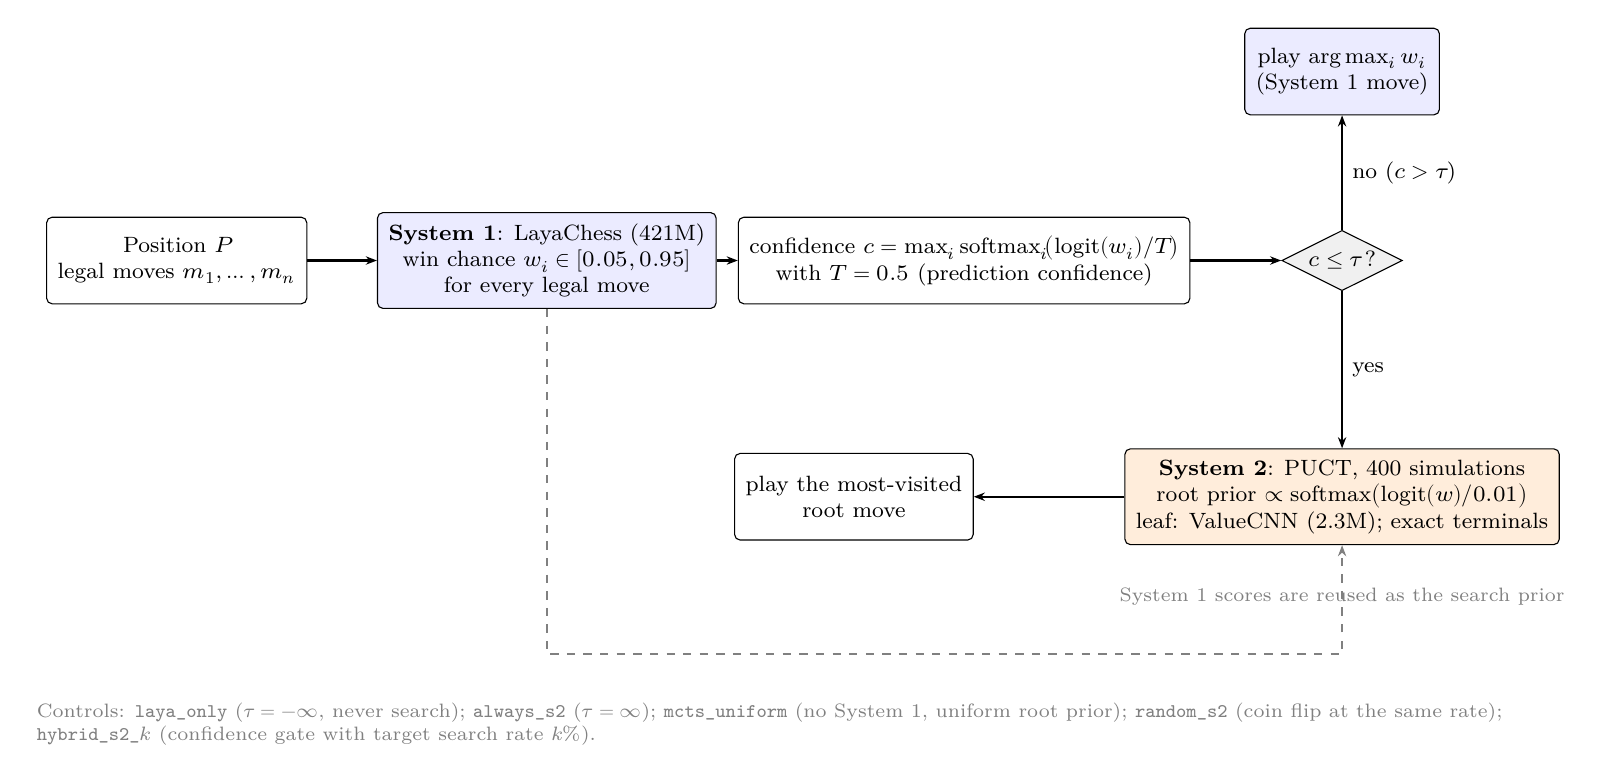
\begin{tikzpicture}[font=\footnotesize,x=1cm,y=1cm,
  box/.style={draw,rounded corners=2pt,align=center,inner sep=4pt,fill=white,minimum height=11mm},
  s1/.style={box,fill=blue!8},s2/.style={box,fill=orange!14},
  gate/.style={draw,diamond,aspect=2,align=center,inner sep=1pt,fill=gray!12},
  arr/.style={-{Stealth[length=4pt]},thick}]
  \node[box] (pos) at (0,0) {Position $P$\\legal moves $m_1,\dots,m_n$};
  \node[s1] (laya) at (4.7,0) {\textbf{System 1}: LayaChess (421M)\\win chance $w_i\in[0.05,0.95]$\\for every legal move};
  \node[box] (conf) at (10.0,0) {confidence $c=\max_i \mathrm{softmax}_i\!\big(\mathrm{logit}(w_i)/T\big)$\\with $T=0.5$ (prediction confidence)};
  \node[gate] (g) at (14.8,0) {$c\le\tau$\,?};
  \node[s1] (play1) at (14.8,2.4) {play $\arg\max_i w_i$\\(System 1 move)};
  \node[s2] (mcts) at (14.8,-3.0) {\textbf{System 2}: PUCT, 400 simulations\\root prior $\propto \mathrm{softmax}\big(\mathrm{logit}(w)/0.01\big)$\\leaf: ValueCNN (2.3M); exact terminals};
  \node[box] (out) at (8.6,-3.0) {play the most-visited\\root move};
  \draw[arr] (pos)--(laya); \draw[arr] (laya)--(conf); \draw[arr] (conf)--(g);
  \draw[arr] (g.north)--node[right]{no ($c>\tau$)}(play1.south);
  \draw[arr] (g.south)--node[right]{yes}(mcts.north);
  \draw[arr] (mcts.west)--(out.east);
  \draw[arr,dashed,gray] (laya.south)--(4.7,-5.0)--(14.8,-5.0)--(mcts.south) node[pos=.35,above,font=\scriptsize,text=gray]{System 1 scores are reused as the search prior};
  \node[font=\scriptsize,gray,align=left,anchor=north west] at (-1.9,-5.5) {Controls: \texttt{laya\_only} ($\tau=-\infty$, never search); \texttt{always\_s2} ($\tau=\infty$); \texttt{mcts\_uniform} (no System 1, uniform root prior); \texttt{random\_s2} (coin flip at the same rate);\\\texttt{hybrid\_s2\_}$k$ (confidence gate with target search rate $k\%$).};
\end{tikzpicture}}
\caption{Neuro-gated chess. System~1 scores every legal move; a threshold on the softmax confidence decides whether the System~1 move is played or the same scores seed a PUCT search. $\tau$ is the validation-set quantile of confidence for the target search rate.}
\label{fig:arch}
\end{figure*}

\subsection{Components (stage V1)}
\textbf{System~1} (learned, external, frozen) is LayaChess (\texttt{datafreak/laya-chess}): one forward pass per legal move returns an expected win chance in $[0.05,0.95]$; it scored \layaScored{} moves per test position. The checkpoint revision was not pinned in V1. \textbf{Confidence and gate} (handcrafted, tuned on validation): confidence is the largest probability of $\mathrm{softmax}(\mathrm{logit}(w_i)/T)$ over legal moves with $T=0.5$. It is a prediction-confidence score, not a calibrated probability: values mostly lie below 0.2 while \goodRateLaya\% of moves are good. The gate sends a position to System~2 iff $c\le\tau$, with $\tau_q$ the validation quantiles of confidence for target rates $q\in\{10,25,50,75\}\%$ (achieved test rates \rateTen, \rateTf, \rateFifty, \rateSf\%). \textbf{System~2} is a PUCT search with 400 simulations, $c_\text{puct}=1.5$, first-play reduction 0.2, no noise or tree reuse; priors are System~1's scores at the root and uniform inside the tree; leaves are scored by a residual value network (18 input planes, six 128-channel blocks, spatial head; \vnParams M parameters) with exact terminals. The final move is the most-visited root move. \textbf{Controls:} \ag{laya_only} (never search), \ag{always_s2}, \ag{mcts_uniform} (no System~1), \ag{random_s2} (coin flip at the same rate) and \ag{hybrid_s2_}$k$ (confidence gate at rate $k\%$).

\textbf{Search is anchored to System~1.} The root-prior temperature was tuned on 150 validation positions: ACPL of \ag{always_s2} was \swTthree{} at 0.3, \swTone{} at 0.1 and \swTz{} at 0.01 (\ag{laya_only}: \swLaya). The chosen 0.01 makes the prior nearly one-hot, so System~2 acts as a verifier that overrides System~1's top move in only \fracChanged\% of test positions. This choice matters for every V1 result and is revisited in Section~\ref{sec:followup}.

\subsection{Extensions in stages V2 and V3}
\label{sec:arch-v2}
After V1 the agent gained the components in Fig.~\ref{fig:arch2}; a move comes from the first stage that decides.

\begin{figure}[t]
\centering
\resizebox{\columnwidth}{!}{%
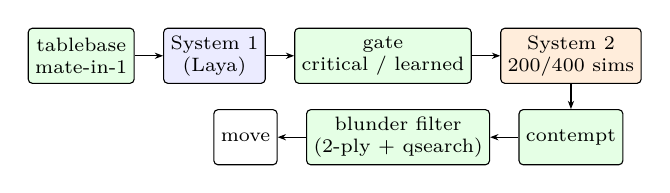
\begin{tikzpicture}[font=\scriptsize,node distance=3.2mm and 3.6mm,
  b/.style={draw,rounded corners=1.5pt,align=center,inner sep=2.5pt,fill=white,minimum height=7mm},
  s1/.style={b,fill=blue!8},s2/.style={b,fill=orange!14},new/.style={b,fill=green!10},
  arr/.style={-{Stealth[length=3pt]}}]
  \node[new] (tb) {tablebase\\mate-in-1};
  \node[s1,right=of tb] (l) {System 1\\(Laya)};
  \node[new,right=of l] (g) {gate\\critical / learned};
  \node[s2,right=of g] (s) {System 2\\200/400 sims};
  \node[new,below=of s] (c) {contempt};
  \node[new,left=of c] (f) {blunder filter\\(2-ply + qsearch)};
  \node[b,left=of f] (m) {move};
  \draw[arr] (tb)--(l); \draw[arr] (l)--(g); \draw[arr] (g)--(s); \draw[arr] (s)--(c); \draw[arr] (c)--(f); \draw[arr] (f)--(m);
\end{tikzpicture}}
\caption{Decision flow of the V2/V3 agent (blue System~1, orange System~2, green added after V1). If the gate does not fire, System~1's move goes straight to contempt.}
\label{fig:arch2}
\end{figure}

\textbf{Blunder filter.} Candidates $\mathcal C$ are the six most preferred moves and all captures. Each gets a material score $M(m)$ from a two-ply full-width search with material-only quiescence, and the agent plays the most preferred move $m^{\ast}$ within $\delta=150$\cp\ of the best:
\begin{equation}
M(m^{\ast})\ge \max_{m'\in\mathcal C} M(m')-\delta .
\end{equation}
It knows nothing about positional quality, deliberately: V1's costliest errors were material. \textbf{Search:} quiescence-corrected leaves, tactical interior priors (MVV-LVA captures, promotions, checks), tablebase leaves, root-prior temperature 0.1. \textbf{Value network:} LeakyReLU head, weight decay $10^{-4}$, labels $\tfrac12 r+\tfrac12\tanh(\mathrm{cp}_{\mathrm{SF}}/400)$. \textbf{Gates:} V2 searches if in check, a piece hangs, a profitable capture exists, there are at most 12 legal moves, or the position is an endgame (400 simulations when sharp, 200 otherwise); V3 uses the logistic model of Section~\ref{sec:followup}. \textbf{Contempt:} if System~1's best win chance is at least 0.55, a repeating move scores as a draw worth $-0.10$ and is replaced by a non-repeating move within 0.06 win chance.

\section{Methods, Data and Statistics}
\label{sec:methods}
\paragraph*{Value network and gate selection}
The V1 value network was trained on about 500{,}000 positions from six months (2025-04 to 2025-09) of the Lichess Elite Database~\cite{lichesselite}, up to eight per game from ply 8, labelled with the game result from White's view, with colour-flip augmentation, AdamW ($10^{-3}$, weight decay $10^{-3}$), cosine decay, ten epochs, and early stopping on 20{,}002 positions of 2025-10. The best epoch reached validation MSE \vnMse{} against 0.811 for the constant predictor and sign accuracy \vnSign\%. The first run overfit after five epochs (MSE 0.703); the change was logged as a deviation, made on validation data only. Candidate confidence functions (margin, top-1 softmax, normalised entropy over $\mathrm{logit}(w)/T$, $T\in\{0.05,0.1,0.2,0.5\}$) were scored on 3{,}000 validation positions by the AUROC with which they separate good moves (CPL $\le25$\cp) from the rest. The top-1 softmax at $T=0.5$ achieved \valAuc{} against 0.585 for the margin and 0.562 for the 1/\#legal-moves baseline and was frozen on 2026-10-18 before any test run.

\paragraph*{Study design}
\emph{Study~A} (main): positions from 2025-11, disjoint by month from training and validation; at most three per game, plies 10--120, stratified into 600 opening, 1{,}800 middlegame and 600 endgame positions (\nPos{} positions from \nGamesA{} games). All agents run on identical positions, so comparisons are paired. Because the gate depends only on System~1's output, each component (\ag{laya_only}, \ag{always_s2}, \ag{mcts_uniform}) is run once per position and hybrids and random gates are composed offline; Study~B plays live agents. \emph{Study~B}: 25 distinct 8-ply openings (judge evaluation within $\pm100$\cp) played with both colours; each agent against a Stockfish anchor (\texttt{UCI\_Elo} 1320, 100\,ms per move) plus six round-robin pairings, 500 games in total. Agents are deterministic, so the opening is the only source of diversity. \emph{Study~C}: 1{,}000 Lichess puzzles~\cite{lichessdb}, 200 in each of five rating buckets. Four deviations from the protocol were logged, none using test results: the prior temperature (0.3 to 0.01), the anchors (planned 1500/1700/1900, replaced by 1320 because \ag{laya_only} already scored 12.5\% against the weakest legal setting), an added round-robin tier, and the value-network settings.

\paragraph*{Judge, metrics and cost}
Stockfish~16 (one thread, 128\,MB, 200{,}000 nodes, \texttt{MultiPV} 2) scores each position from the side to move's view, mate scores map to $\pm1000$\cp\ and scores are clipped there. Centipawn loss is $\mathrm{CPL}(m)=\max(0,s^*-s(m))$; ACPL is its mean; a \emph{good} move has CPL $\le25$\cp, a \emph{blunder} $\ge200$\cp. ACPL is dominated by a minority of large errors (median CPL \medLaya\cp\ for \ag{laya_only}, mean \acplLaya\cp). Cost is wall-clock time per move on one RTX~4060 laptop GPU under WSL2 (PyTorch 2.14.1, \texttt{python-chess} 1.11.2~\cite{pythonchess}), with System~1's cache disabled. System~1 is not cheap: it costs \msLayaPart\,ms per position against \msSearch\,ms for a 400-simulation search, so the gate decides when to add search on top of a pass that is always paid.

\paragraph*{Statistics}
Study~A intervals are 95\% percentile bootstraps over positions (2{,}000 resamples), resampling positions jointly across agents. \Htwo{} is evaluated at the \emph{achieved} test rate by a one-sided paired bootstrap with Holm correction over 25\% and 50\%. The protocol redraws the random gate inside every resample, which adds noise (about \randSd\cp); as a sensitivity analysis we also use the expectation over random gates, where the per-position benefit over a random gate at rate $r$ is $(m_i-r)\,g_i$ with $m_i\in\{0,1\}$ the gate decision and $g_i=\mathrm{CPL}_{S1,i}-\mathrm{CPL}_{S2,i}$ the search gain. Game-clustered bootstraps check dependence between positions. Ratings are Bradley--Terry maximum pseudo-likelihood estimates~\cite{bradley1952,hunter2004,elo1978} with draws as half-wins, the anchor fixed at 1320 and cluster-bootstrap intervals over openings~\cite{efron1979}; they are anchor-relative, not absolute. Puzzle differences use exact McNemar tests~\cite{mcnemar1947} and Wilson intervals~\cite{wilson1927}. A non-significant difference does not establish equivalence, so we also report the minimum detectable advantage at 80\% power ($2.8\times$ the standard error). Every V1 statistic was reproduced from raw files (\nChecksOk{} of \nChecks{} checks against the project's published numbers).

\section{Results: Stage V1}
\label{sec:results}
All numbers come from the reproduction script on the original result files. Study~A has \nPos{} paired positions, Study~B 500 games and Study~C 1{,}000 puzzles.

\subsection{Search versus System~1 alone (descriptive)}
\label{sec:search-value}
Always searching lowers ACPL from \acplLaya{} to \acplSTwo{}: a paired difference of \dAcpl{}\cp\ (95\% CI [\dAcplLo, \dAcplHi]; [\dClLo, \dClHi] resampling games) at \costRatio$\times$ the cost (\msLaya\ to \msSTwo\,ms; Table~\ref{tab:agents}). The standardised effect is small ($d_z=\cohenDz$). Blunders fall from \blunLaya\% to \blunSTwo\%. \ag{mcts_uniform}, the value network without System~1, is far worse (ACPL \acplMcts{}), so search is useful only because it inherits System~1's scores. The average is carried by a minority of positions: search changes System~1's move in \fracChanged\% (\nChanged{}); of these \nBetter{} are better, \nWorse{} worse and \nEqual{} equal. Capping CPL at 200\cp\ shrinks the difference to \capTwoHundred\cp, and search repairs \nFixed{} of \nLayaBlunder{} System~1 blunders (\fixedPct\%) while introducing \nIntro{} new ones.

\begin{table}[t]
\centering
\caption{Study~A (test split, $n=\nPos$ positions per agent). System~1 = \ag{laya_only}, Always~S2 = \ag{always_s2}, MCTS only = \ag{mcts_uniform}; time is mean wall time per move.}
\label{tab:agents}
\small
\footnotesize\setlength{\tabcolsep}{4pt}\begin{tabular}{lrrr}
\toprule
 & System 1 & Always S2 & MCTS only \\
\midrule
ACPL (cp) & 107.9 & 103.1 & 235.4 \\
\quad 95\% CI & [101.0, 114.4] & [96.6, 109.6] & [226.0, 245.0] \\
Median CPL (cp) & 28 & 26 & 121 \\
Good moves (\%) & 48.6 & 49.7 & 31.2 \\
Blunders (\%) & 17.3 & 16.6 & 42.4 \\
Top-1 agreement (\%) & 26.2 & 27.0 & 17.7 \\
Mean ms per move & 468 & 1499 & 1042 \\
\bottomrule
\end{tabular}

\end{table}

\subsection{Is confidence informative? (\Hone{}, \Hfour{})}
The AUROC of confidence for predicting a good move is \aucConf{} [\aucConfLo, \aucConfHi], close to its validation value (\valAuc{}); it exceeds the legal-move baseline (\aucBase{}) only by \aucDiff{} [\aucDiffLo, \aucDiffHi], an interval including zero, so \Hone{} is met only in its first clause. The good-move rate rises with confidence from about 42\% to 91\%. \Hfour{} fails in the opposite direction: the blunder rate is \qOne\% in the lowest-confidence quartile and \qFour\% in the highest (ratio \qRatio{} [\qRatioLo, \qRatioHi]). One post hoc reading is that low-confidence positions have many near-equal moves, so errors there are cheap, whereas large errors concentrate in sharp positions: \ag{laya_only} has ACPL \acplSharp\cp\ where the Stockfish gap exceeds 300\cp, and its mean confidence there is \confSharp{} against \meanConfAll{} overall.

\subsection{Does confidence gating beat random gating? (\Htwo{}, \Hthree{})}
\label{sec:h2}
\begin{figure*}[t]
\centering
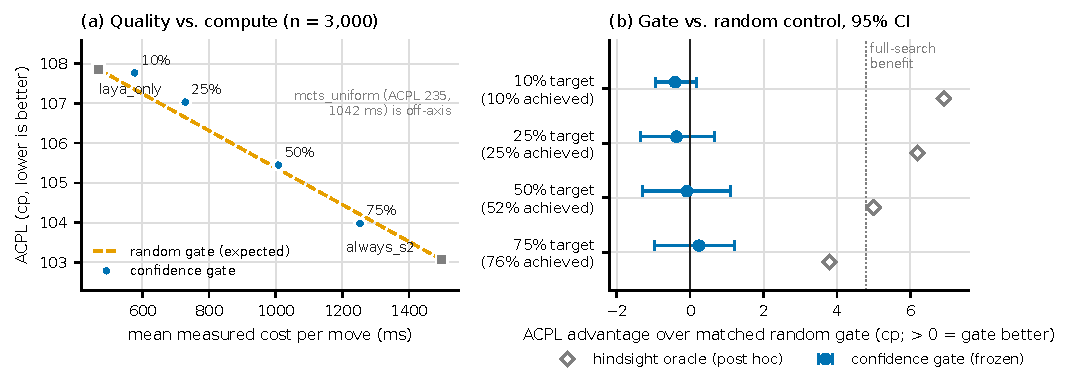
\includegraphics[width=\textwidth]{fig_tradeoff}
\caption{Quality--compute trade-off, Study~A. (a) ACPL against measured cost for the frozen confidence gate at its four achieved rates; the dashed line is the expected value of a random gate. (b) ACPL advantage of the confidence gate over a random gate at the same rate (analytic expectation; 95\% bootstrap interval). Hollow diamonds are a post hoc hindsight oracle and are not achievable.}
\label{fig:tradeoff}
\end{figure*}
\begin{table*}[t]
\centering
\caption{\Htwo{} and \Hthree{} at the frozen thresholds (Study~A). $^{\dagger}$Expectation over random gates at the achieved rate. Advantage $>0$ favours the confidence gate. Recovery $R=(\mathrm{ACPL}_{S1}-\mathrm{ACPL}_{gate})/(\mathrm{ACPL}_{S1}-\mathrm{ACPL}_{S2})$; a random gate has expected $R$ equal to its search rate.}
\label{tab:h2}
\small
\begin{tabular}{rrrrcccr}
\toprule
Target & Achieved & ACPL & ACPL & Gate $-$ random advantage & Holm & Recovery $R$ & Search time \\
rate (\%) & rate (\%) & gate & random$^{\dagger}$ & (cp, 95\% CI) & $p$ & [95\% CI] & used (\%) \\
\midrule
10 & 10.5 & 107.77 & 107.35 & \ensuremath{-}0.41 [\ensuremath{-}0.96, 0.17] & -- & 0.02 [\ensuremath{-}0.13, 0.15] & 10.5 \\
25 & 25.0 & 107.03 & 106.66 & \ensuremath{-}0.37 [\ensuremath{-}1.37, 0.67] & 1.00 & 0.17 [\ensuremath{-}0.06, 0.40] & 25.2 \\
50 & 52.1 & 105.45 & 105.36 & \ensuremath{-}0.09 [\ensuremath{-}1.30, 1.11] & 1.00 & 0.50 [0.24, 0.79] & 52.3 \\
75 & 75.9 & 103.98 & 104.22 & 0.24 [\ensuremath{-}0.96, 1.22] & -- & 0.81 [0.56, 1.04] & 76.2 \\
\bottomrule
\end{tabular}

\end{table*}
At no rate does the gate beat its matched random control (Fig.~\ref{fig:tradeoff}, Table~\ref{tab:h2}). At the two pre-registered rates the advantage is \advTf{}\cp\ [\advTfLo, \advTfHi] at \rateTf\% and \advFifty{}\cp\ [\advFiftyLo, \advFiftyHi] at \rateFifty\%; both Holm-adjusted $p$-values are 1.0, so \Htwo{} is not supported. The 10\% and 75\% rates agree (\advTen{}, \advSf{}\cp). The absence of an advantage is not equivalence: the minimum detectable advantage is \mdeTen--\mdeFifty\cp, and the data are compatible with an advantage of up to \maxAdvHi\cp\ (\maxAdvHiPct\% of the full benefit). \Hthree{} is not supported: at \rateFifty\% search the gate recovers $R=\RFifty$ [\RFiftyLo, \RFiftyHi] of the benefit, but uses \shareFifty\% of the search time and a random gate is expected to recover $R=\randRFifty$. Recovery is proportional to the search budget.

\subsection{Playing strength (\Hsix{}) and puzzles (\Hfive{})}
\label{sec:studyb}
\begin{table}[t]
\centering
\caption{Study~B ratings on the anchor's nominal scale, pooled over all 500 games (anchor 1320 fixed). Each agent played 200 games; the last column is its score in the 50 games against the anchor (Wilson interval).}
\label{tab:elo}
\small
\footnotesize\setlength{\tabcolsep}{3pt}\begin{tabular}{lrrr}
\toprule
Agent & Elo$^{\ddagger}$ [95\% CI] & Score (\%) & vs.\ anchor (\%) \\
\midrule
\texttt{laya\_only} & 904 [832, 958] & 46.8 & 11 (5--23) \\
\texttt{always\_s2} & 887 [821, 938] & 44.2 & 6 (2--16) \\
\texttt{hybrid\_s2\_50} & 879 [809, 932] & 43.0 & 8 (3--19) \\
\texttt{mcts\_uniform} & 734 [668, 783] & 22.5 & 1 (0--9) \\
\bottomrule
\end{tabular}

\end{table}
Ratings (Table~\ref{tab:elo}) are \ag{laya_only} \eloLaya{} [\eloLayaLo, \eloLayaHi], \ag{always_s2} \eloAlw{}, \ag{hybrid_s2_50} \eloHyb{}, \ag{mcts_uniform} \eloMu{}. The paired contrast for \Hsix{} is \eDHL{} Elo [\eDHLLo, \eDHLHi] for hybrid minus \ag{laya_only}: the estimate favours System~1 alone, from three decisive head-to-head losses of the hybrid and none won (\hhWins{} wins, \hhDraws{} draws, \hhLosses{} losses), so we read it as weak evidence against \Hsix{}, not as evidence that the hybrid is weaker. Three qualifications apply. Every agent scored only \ancMu--\ancLaya\% against the single anchor, so absolute ratings are extrapolations. \rrThree{} of \rrN{} round-robin games (\rrThreePct\%) ended in threefold repetition and only \nUniqSeq{} distinct move sequences occur among 500 games, so the effective number of games is well below 500. And in games \ag{hybrid_s2_50} used System~2 on \hybSysShare\% of moves, far above its \rateFifty\% rate in Study~A, because game positions have low confidence.

On puzzles, search adds little: pooled solve rates are \puzPoolLaya\% for \ag{laya_only}, \puzPoolHyb\% for \ag{hybrid_s2_50} and \puzPoolAlw\% for \ag{always_s2} (paired difference \puzDAlw{} points [\puzDAlwLo, \puzDAlwHi], McNemar $p=\puzPAlw$), and no bucket differs by more than \puzMaxBucket{} points. This bounds the effect to one or two points; it does not show search is useless on tactics. \Hfive{} fails in the opposite direction: the 50\% gate sends \trigPuz\% of puzzles to search against \trigGames\% of game positions, plausibly because forcing positions have a standout top move and hence high confidence.

\subsection{Exploratory: why confidence fails to locate search gains}
\label{sec:explore}
Everything here was computed after the test outcomes were visible and changes no verdict. Low confidence flags where search \emph{changes} the move (AUROC \aucChange; override rate \decChangeLow\% in the least confident decile against \decChangeHigh\% in the most), but among changed positions it does not predict improvement (AUROC \aucImprove, Spearman $\rho=\rhoChanged$), and the average gain of an override is larger where System~1 is confident (\chGainHigh\cp\ against \chGainLow\cp). Overall, confidence and search gain have $\rho=\rhoGain$ [\rhoGainLo, \rhoGainHi], with \fracGainZero\% of gains exactly zero. Gains concentrate in endgames (\gainEnd\cp, Holm $p=\pHolmEnd$) and in positions where one move is more than 300\cp\ better than the next (\gainSharp\cp, $n=\nSharp$, Holm $p=\pHolmSharp$); positions with gap above 300\cp\ (\fracSharp\%) supply \shareSharp\% of total gain. These are the positions where System~1 is \emph{more} confident, so confidence behaves as a forcedness signal and a gate that triggers on low confidence points away from where search helps. Gates on inverted confidence, legal-move count or even the Stockfish gap stay within about 1\cp\ of random. A hindsight oracle reaches ACPL \oracleAcpl{} at a 10\% rate (\oracleCostPct\% of the cost of always searching), below always searching (\acplSTwo{}), but it is selected and scored on the same noisy judgments, so it is a ceiling and not an achievable gate.

\section{Follow-up Stages: Repairing the Agent and Re-testing the Gate (V2, V3)}
\label{sec:followup}
\paragraph*{Progression and evidence status}
Sections~\ref{sec:hyp}--\ref{sec:explore} report stage~V1, the pre-specified confidence-gate study. Its negative result changed the project's question in two steps. V2 asked whether fixing the weaknesses that V1 exposed makes the agent stronger, and which fix matters. V3 returned to the original question with a better gate and added a control for whether System~1 contributes at all once V2's repairs exist. V1 is retained unchanged as the confirmatory study; V2 and V3 each have their own protocol (\path{docs/V2_PROTOCOL.md}, \path{docs/V3_PROTOCOL.md}) committed before the corresponding test runs, with the same self-registration caveat as in Section~\ref{sec:hyp}.

The three stages are not directly comparable. Each used a different, previously unused test month, a different number of positions, a different opening set and (in V3) a different anchor set (Table~\ref{tab:stages}). ACPL and Elo are therefore compared \emph{within} a stage, never across stages. V1 was reproduced from its raw result files. For V2 and V3 we recomputed the move-quality, gate and rating statistics from the per-position and per-game files of the development laptop (84 numerical checks, none failed; Appendix~\ref{app:evidence}), using the project's own Elo code and the frozen gate weights. Two kinds of quantity were not recomputed: development-stage figures that appear only in the deviations log and protocols, and the learned-gate cross-validation figures.

\begin{table*}[t]
\centering
\caption{The three stages. Test positions and openings are disjoint between stages and from all development data. ``Evidence'' states what we could check; Appendix~\ref{app:evidence} gives details. $^{\natural}$Elo values are on an anchor-relative scale that is not shared across stages.}
\label{tab:stages}
\small
\begin{tabular}{@{}>{\raggedright\arraybackslash}p{0.8cm}>{\raggedright\arraybackslash}p{3.2cm}>{\raggedright\arraybackslash}p{5.2cm}>{\raggedright\arraybackslash}p{3.5cm}>{\raggedright\arraybackslash}p{3.2cm}@{}}
\toprule
 & Question & Agent changes & Test data & Evidence \\
\midrule
V1 & Does System~1 confidence tell when to search? & Confidence gate (Section~\ref{sec:arch}) & 2025-11; 3{,}000 positions; 25 openings; anchor 1320; 500 games & Reproduced from raw files (70 checks) \\
V2 & Can targeted fixes make the agent stronger? & Blunder filter, tablebases, mate-in-one, contempt, quiescence leaves, tactical priors, hand-written criticality gate, retrained value net & 2025-03; 2{,}000 positions; 50 openings; anchor 1320; 600 games & Recomputed from per-position and per-game files \\
V3 & Can a learned gate decide when to search? Does System~1 matter? & Logistic gate over 18 pre-search features; classical-policy control; second anchor & 2025-02; 2{,}000 positions; 50 openings; anchors 1320, 1600; 800 games & Recomputed from per-position and per-game files \\
\bottomrule
\end{tabular}
\end{table*}

\subsection{V2: repairing the diagnosed weaknesses}
\paragraph*{Design}
Each V2 component answers one V1 finding: 17.3\% of System~1 moves were blunders that search barely repaired (blunder filter); leaves were evaluated mid-exchange and interior priors were uniform (quiescence, tactical priors); confidence did not locate search gains, which lay in sharp positions and endgames (criticality gate); the value network was constant on 9.2\% of test positions (retrained); search helped most in endgames (tablebases, mate-in-one); and 74\% of round-robin games ended in repetition (contempt). Only the root-prior temperature was tuned. The decision flow is in Section~\ref{sec:arch-v2}. V2 was developed on V1 validation positions and V1 openings only, then frozen before the fresh-month runs (tag \texttt{v2-frozen}).

\paragraph*{Development decisions and deviations}
The retrained value network met the pre-specified Spearman criterion against Stockfish on validation (0.665 against 0.619 for the V1 network) but missed the dead-head criterion (1.3\% against the required $<1\%$). With a LeakyReLU head an inactive hidden layer no longer forces a constant output, and the constant-output rate was 0.0\% (V1 network on the same check: 8.1\%); the network was accepted and the miss logged. The root-prior temperature was chosen on the first 300 validation positions, ACPL 75.3 at 0.01 against 68.8 at 0.1, so 0.1 was frozen. This choice used the same positions that report it and the figures are optimistic. The first launch of the V2 tournaments exhausted memory before any game was played and was relaunched as two staggered processes; no result was affected.

\paragraph*{Move quality (Study~A-v2)}
On 2{,}000 fresh positions, the blunder filter alone (\ag{v2_safe}, no search) lowers ACPL from 114.5 to 76.5 and the blunder rate from 17.7\% to 11.5\% (Table~\ref{tab:v2a}). Adding the criticality gate and the improved search (\ag{v2_full}) lowers ACPL to 68.7, and searching on every move (\ag{v2_always}) to 65.4. The three differences from System~1 alone have paired 95\% intervals that exclude zero. Paired intervals between V2 agents, recomputed from the per-position data, are $-7.8$\cp\ [$-11.7$, $-4.2$] for \ag{v2_full} against \ag{v2_safe}, $-3.3$ [$-5.5$, $-1.1$] for \ag{v2_always} against \ag{v2_full}, and $+1.0$ [$-1.1$, $+3.1$] for the old network against the retrained one. The 7.8\cp\ gain from search and gating on top of the filter is therefore distinguishable from zero, but it bundles several changes (criticality gate, quiescence, tactical priors, temperature 0.1, new value network) that were not separated experimentally. On top of the filter, search helps in endgames (ACPL 64.5 to 53.8) and middlegames (91.8 to 82.0) and does not help in openings (42.5 to 43.5); by-phase figures are from the project's \path{V2_studyA_by_phase.csv}.

\begin{table}[t]
\centering
\caption{Study~A-v2 (fresh month 2025-03, 2{,}000 positions per agent; read from result files). Bl.\ is the blunder rate, S2 the share of moves searched, ms the mean time per move, and $\Delta$ACPL the paired difference from \ag{laya_only} (bootstrap over positions). $^{\dagger}$Added post hoc after the tournament, on the same positions.}
\label{tab:v2a}
\scriptsize\setlength{\tabcolsep}{2.2pt}\begin{tabular}{lrrrrr}\toprule
Agent & ACPL & Bl.\ \% & $\Delta$ACPL [95\% CI] & S2 \% & ms \\
\midrule
\texttt{laya\_only} & 114.5 & 17.7 & -- & 0 & 476 \\
\texttt{v2\_safe} & 76.5 & 11.5 & -38.1 [-44.9, -31.2] & 0 & 571 \\
\texttt{v2\_full} & 68.7 & 9.6 & -45.9 [-53.6, -38.2] & 60 & 1308 \\
\texttt{v2\_always} & 65.4 & 9.2 & -49.1 [-57.2, -41.2] & 99 & 1604 \\
\texttt{v2\_full\_oldnet}$^{\dagger}$ & 69.7 & 9.7 & -44.8 [-52.4, -37.3] & 60 & 1166 \\
\bottomrule\end{tabular}

\end{table}

\paragraph*{Playing strength (Tournament-v2)}
Against the 1320 anchor, \ag{v2_full} scored 25.0\% against 9.5\% for \ag{laya_only}, and beat \ag{laya_only} head-to-head by 76 points to 24 over 100 games. Table~\ref{tab:stageelo} places it about 200 Elo above \ag{laya_only} (1130 against 930). The \ag{laya_only} rating is flagged off-scale because it scored under 10\% against the only anchor, so the size of the gap is an extrapolation although its direction is not in doubt. Games ended by threefold repetition in 142 of 600 cases against 74.3\% of V1 round-robin games, but V1's figure came from games between our own deterministic agents, so the two are not comparable. Whether contempt caused the drop was not tested (its ablation was not run).

Two ablations bear on what matters. The V1 value network inside the V2 agent (\ag{v2_full_oldnet}) is statistically indistinguishable from the retrained one: 1.0\cp\ worse in Study~A and 39 Elo higher in games, both well inside the intervals. The agent's strength no longer depends visibly on the value network. Removing the blunder filter from \ag{v2_full} (\ag{v2_full_nosafety}) leaves 1080 Elo, roughly equal to the filter without search (\ag{v2_safe}, 1069), with 100 games each and intervals of about $\pm70$ Elo. The project's summary that the blunder filter ``gives most of the gain'' is supported for move quality (Study~A) but not isolated for playing strength: \ag{v2_safe} also contains tablebases, mate-in-one and contempt, and \ag{v2_full_nosafety} retains them, so neither pair of agents separates the filter from those rules.

\paragraph*{Scrutiny of the V2 gate (post hoc)}
V1's negative result raised the question of whether the criticality gate also fails the matched-random control, which V2 had not included. A post hoc script reported that the criticality gate at its 60\% search rate is not distinguishable from a random gate at the same rate ($+1.1$\cp, 95\% CI $[-2.4,+4.7]$), while a hindsight oracle at that rate would reach ACPL 52.6 against 68.7. We reproduced these figures from the per-position data (point estimate $+1.10$, oracle 52.6, interval $[-2.3,+4.8]$ with the same fresh-random-gate procedure). With the lower-variance analytic comparison used below the interval is $[-0.8,+3.1]$, which still contains zero.

\subsection{V3: a learned gate, a classical control and a second anchor}
\paragraph*{Design}
The V3 gate is a logistic model $g(\mathbf{x})=\sigma(\mathbf{w}^{\top}\mathbf{x}+b)$ that predicts whether searching improves the move, i.e.\ whether $\mathrm{CPL}_{\text{safe}}-\mathrm{CPL}_{\text{always}}>0$. It takes 18 features available before search (System~1 win-chance margins, entropy and confidence, legal-move and capture counts, the five criticality flags, material, ply, whether the filter overrides System~1, two tactical-score summaries) and was trained on the 3{,}000 V1 validation positions with five-fold cross-validation grouped by game; a ridge model was the alternative. Thresholds for 10\%, 25\% and 60\% search rates were set on validation. The largest weights favour search when System~1 cannot separate its top moves (margin $-1.76$, confidence $-1.28$), the same direction as V1's confidence gate. Composed validation ACPL under cross-validation was 74.2/71.7/68.3 for the learned gate against 76.5/74.6/70.2 for a random gate at 10/25/60\%.

Two V3 engine options were tested on validation positions against rules fixed in advance (adopt only if $\ge2$\cp\ better and $\le30\%$ slower) and rejected: extending the filter's search with checks (0.3\cp), and a System~1 two-ply look-ahead (1.4--4.8\cp\ for 27--59\% more time). The look-ahead was run on the test set as the labelled exploratory agent \ag{v3_look4}, ACPL 64.5 (Study~A only).

The tournament added \ag{classical_full}, the same filter and search driven by a hand-written heuristic policy instead of System~1, to test whether System~1 matters once the filter exists, and a second anchor at Elo 1600.

\paragraph*{An invalid first run, reported}
The first V3 test run was invalid. The generated configuration had silently reset the root-prior temperature to 0.01, V1's value, overwriting the V2 choice (0.1), because a later code handoff replaced the generator script. Search then agreed with the filter's move on 92.8\% of positions and gained 1.55\cp\ on average instead of 11.7\cp\ in the valid re-run (both recomputed from the saved files; the re-run agrees on 55\% of positions). The run (kept as \texttt{v3\_bench\_T001\_INVALID}) yielded a learned-gate advantage of only $+0.5$ to $+0.7$\cp\ over random, and did not test the frozen design. The setting was restored and Study~A and the tournaments were re-run on the same 2025-02 sets with the same frozen gate. The invalid result had been seen before the re-run, and we report both. The failure is informative: a root-prior temperature of 0.01 makes search nearly inert, which supports the reading of V1's small search effect (8.2\% of moves changed) offered in Section~\ref{sec:arch}, although V1 never tested that link directly.

\paragraph*{Gate results (Q1)}
The pre-specified primary question was whether the learned gate beats a random gate at the same rate, tested at 25\% with Holm correction over 10/25/60\%. Under the pre-registered procedure it does not (Table~\ref{tab:v3gate}, left block): the advantage is $+2.5$\cp\ [$-0.9$, $+5.8$], $p=0.069$, and after Holm adjustment no rate is significant. We reproduced these figures exactly from the per-position data and the frozen gate weights. That procedure draws a fresh random gate inside every bootstrap resample, so its interval includes the sampling noise of one random mask. This is the same noise that the V1 analysis removed by using the expectation over random gates (Section~\ref{sec:methods}).

Applying that expectation-based (analytic) test to the same V3 data, a post hoc analysis that was not pre-specified, gives narrower intervals (Table~\ref{tab:v3gate}, right block): $+2.5$\cp\ [$+0.4$, $+4.7$] at 25\% (Holm $p=0.021$) and $+3.2$\cp\ [$+1.4$, $+4.9$] at 60\% (Holm $p<0.001$), with the 10\% rate not significant ($p=0.063$). Resampling the 1{,}696 games instead of positions leaves this unchanged (25\%: $[+0.4,+4.6]$). The point estimates are identical in the two analyses; only the width of the interval differs. We therefore report both: the pre-registered verdict, that the primary comparison is not supported, stands, and the post hoc analysis indicates a real but modest advantage over random gating of about 2.5\cp\ at a 25\% rate. The learned gate closes about 12\% of the gap between a random gate and the hindsight oracle at 25\% ($2.5/20.2$\cp). The same analytic test also puts the hand-written criticality gate ahead of random on the V3 positions ($+2.5$\cp\ [$+0.6$, $+4.5$] at its 57.6\% rate) but not on the V2 positions ($+1.1$ [$-0.8$, $+3.1$] at 60\%), so the evidence for a learned gate over a hand-written one is not established, and we did not test them against each other.

\begin{table*}[t]
\centering
\caption{V3 test, composed ACPL on 2{,}000 positions of 2025-02, recomputed from the per-position files. Advantage is random minus learned (cp; $>0$ favours the learned gate); $p$ is one-sided; Holm over the three rates. Pre-registered test: a fresh random gate per resample (reproduces the project's logged output). Analytic test (post hoc): expectation over random gates, 4{,}000 position resamples. Reference ACPL: never search 76.6, critical gate (57.6\%) 67.4, always search 64.9. $^{*}$Primary comparison. $^{\S}$Hindsight oracle, not achievable.}
\label{tab:v3gate}
\scriptsize\setlength{\tabcolsep}{2.2pt}\begin{tabular}{rrrrrrrrrr}\toprule
 & & & & \multicolumn{3}{c}{Pre-registered test} & \multicolumn{3}{c}{Analytic test (post hoc)} \\
\cmidrule(lr){5-7}\cmidrule(lr){8-10}
Rate (\%) & Learned & Random & Oracle$^{\S}$ & Advantage [95\% CI] & $p$ & Holm & Advantage [95\% CI] & $p$ & Holm \\
\midrule
10 & 74.1 & 75.4 & 57.1 & +1.3 [-1.2, +3.9] & 0.149 & 0.149 & +1.3 [-0.3, +3.1] & 0.063 & 0.063 \\
25$^{*}$ & 71.1 & 73.6 & 53.4 & +2.5 [-0.9, +5.8] & 0.069 & 0.138 & +2.5 [+0.4, +4.7] & 0.010 & 0.021 \\
60 & 66.4 & 69.6 & 53.4 & +3.2 [+0.1, +6.7] & 0.022 & 0.066 & +3.2 [+1.4, +4.9] & $<$0.001 & $<$0.001 \\
\bottomrule\end{tabular}

\end{table*}

\paragraph*{Strength and the role of System~1 (Q2--Q4)}
Table~\ref{tab:stageelo} and Table~\ref{tab:v3diff} give the V3 ratings and the paired differences (a shared bootstrap over openings, computed by a script written after the run because per-agent intervals cannot be subtracted). In games the learned gate searched on 39.8\% of moves, not the 25\% it was calibrated for, because positions arising in play look uncertain to it more often than benchmark positions; the same effect appeared for the V1 gate (Section~\ref{sec:studyb}). It matched \ag{v2_full} in rating ($-3$ Elo) at about 20\% less time per move (0.91 against 1.13 s), but the interval ($-89$ to $+81$) is far too wide to show equivalence, so Q2 is inconclusive. Replacing System~1 by the hand-written policy costs about 212 Elo [133, 296] (Q3), so System~1 does contribute, and the filter overrode the heuristic policy on 35.7\% of its moves against 9\% for System~1-driven \ag{v2_full}. The V2 comparison replicates on a second month and under two anchors: \ag{v2_full} is 289 Elo [208, 380] above \ag{laya_only} (Q4), with Study~A ACPL $111.8\to67.4$ and blunders $17.4\%\to9.7\%$, close to V2's $114.5\to68.7$ and $17.7\%\to9.6\%$. Study~A did not run the live \ag{v3_learned_25} and \ag{classical_full} agents; the learned gate's ACPL is the offline composition from the other agents' moves.

\begin{table}[t]
\centering
\caption{Ratings by stage. Elo is anchor-relative and each panel has its own opponents and openings; compare differences within a panel only. $^{\ddagger}$Scored under 10\% against the anchor (off-scale). Each V3 agent played 100 games against each of two anchors; the last two columns give its score against each.}
\label{tab:stageelo}
\scriptsize\setlength{\tabcolsep}{2.2pt}\begin{tabular}{lrrrr}\toprule
Agent & Elo [95\% CI] & Games & vs.\ 1320 (\%) & vs.\ 1600 (\%) \\
\midrule
\multicolumn{5}{l}{\textit{V2, test month 2025-03; anchor 1320 only}}\\
\texttt{laya\_only}$^{\ddagger}$ & 930 [863, 984] & 200 & 9.5 & -- \\
\texttt{v2\_safe} & 1069 [1005, 1125] & 100 & 19.0 & -- \\
\texttt{v2\_full\_nosafety} & 1080 [998, 1148] & 100 & 20.0 & -- \\
\texttt{v2\_full} & 1130 [1072, 1180] & 200 & 25.0 & -- \\
\texttt{v2\_full\_oldnet} & 1169 [1090, 1235] & 100 & 29.5 & -- \\
\midrule\multicolumn{5}{l}{\textit{V3, test month 2025-02; anchors 1320 and 1600}}\\
\texttt{laya\_only}$^{\ddagger}$ & 903 [825, 966] & 200 & 7 & 3 \\
\texttt{classical\_full} & 980 [912, 1036] & 200 & 11 & 4 \\
\texttt{v2\_full} & 1192 [1145, 1236] & 200 & 26 & 15 \\
\texttt{v3\_learned\_25} & 1189 [1128, 1251] & 200 & 24.5 & 16 \\
\bottomrule\end{tabular}

\end{table}

\begin{table}[t]
\centering
\caption{V3 paired Elo differences. Q2: inconclusive, since the interval includes $-50$.}
\label{tab:v3diff}
\scriptsize\setlength{\tabcolsep}{2.2pt}\begin{tabular}{lrl}\toprule
Contrast & $\Delta$Elo [95\% CI] & Status \\
\midrule
v3\_learned\_25 $-$ v2\_full & -3 [-89, +81] & Q2 \\
v2\_full $-$ classical\_full & +212 [+133, +296] & Q3 \\
v2\_full $-$ laya\_only & +289 [+208, +380] & Q4 \\
classical\_full $-$ laya\_only & +76 [-33, +190] & exploratory \\
\bottomrule\end{tabular}

\end{table}

\begin{figure*}[t]
\centering
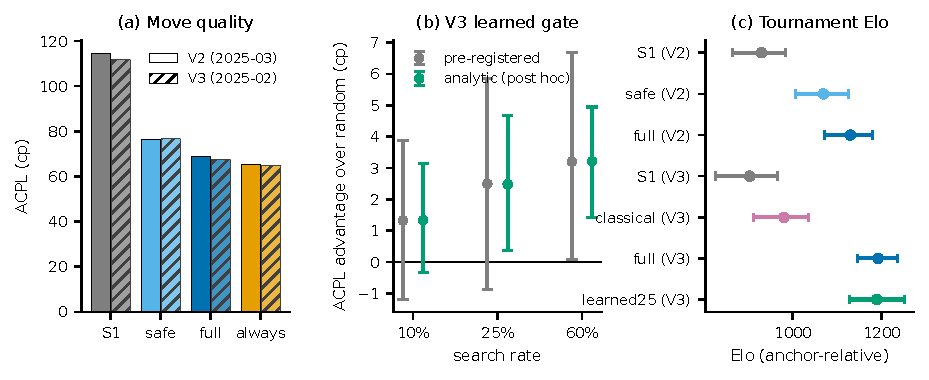
\includegraphics[width=\textwidth]{fig_stages}
\caption{Stages V2 and V3 (different test months and opponents; compare within an agent family, not across stages). (a) ACPL. S1 is \ag{laya_only}, safe is the blunder filter without search, full adds the gate and search, always searches on every move. (b) V3 learned-gate ACPL advantage over a random gate with 95\% intervals under the pre-registered and the analytic (post hoc) procedures; the point estimates are the same. (c) Tournament Elo with 95\% cluster-bootstrap intervals against Stockfish anchors; S1 is off-scale in both stages.}
\label{fig:stages}
\end{figure*}

\subsection{Three gates, one partial answer}
Across the three stages the gating question received a mostly negative and, in the last stage, a modest positive answer. The V1 confidence gate was $-0.09$\cp\ [$-1.30$, $+1.11$] from random at a 52\% rate, under the expectation-based comparison. The V2 criticality gate was $+1.1$\cp\ [$-0.8$, $+3.1$] at 60\% (post hoc). The V3 learned gate was $+2.5$\cp\ at 25\%: not significant under the pre-registered test ($p=0.069$) and significant under the post hoc analytic test ($[+0.4,+4.7]$). These comparisons use different systems, test sets and rates, and only V1 and the V3 primary comparison were pre-specified, so they are not a sequence of improvements. The learned gate has the clearest evidence of an advantage over random gating among the gates studied, but it recovers only about an eighth of the oracle headroom, and what produced a large gain was not a gate but a shallow material check in front of System~1.

\section{Discussion}
\label{sec:disc}
\paragraph*{What the experiments establish}
For stage V1, three statements are well supported. (1) Search on top of System~1 improves mean move quality modestly (\dAcplAbs\cp, about \fixedPct\% of System~1's blunders repaired) at \costRatio$\times$ the cost, through a small share of positions with large corrections. (2) System~1's confidence is weakly informative about whether its move is good (AUROC \aucConf) and does not identify where search helps: the confidence gate is indistinguishable from random gating at four rates, and two further predictions (\Hfour{}, \Hfive{}) are contradicted. (3) The V1 hybrid is not shown to be stronger than System~1 alone. The data do not show that the gate is useless, only that any advantage is below about \maxAdvHi\cp, and they do not show that selective search cannot work: the oracle indicates a perfect selector would exceed the full-search benefit while searching a few percent of positions, so what failed was one particular selector.

\paragraph*{Predictive uncertainty is not decision-criticality}
The exploratory evidence suggests a mechanism, offered as a hypothesis. Search helps rarely (\fracGainPos\% of positions improve) and in a heavy-tailed way: a few percent of positions, mostly forcing, endgame or tactically sharp, account for the net gain. There the model's ranking is sharply peaked, so confidence is \emph{high}, while positions with a flat ranking have little to gain. A confidence gate therefore sends compute where search changes the move often but with little net benefit. This is the difference between $P(\text{wrong})$, which confidence estimates, and $P(\text{search changes the move})\times\text{gain}$, which a router needs. Better-calibrated uncertainty~\cite{lakshminarayanan2017,gal2016} would improve the first without necessarily helping the second.

\paragraph*{What the follow-up stages change}
The follow-up alters the practical picture without overturning the V1 verdict. First, the largest improvement in move quality came from a component that is not a gate: a material-only blunder filter cut ACPL by 38\cp\ on fresh positions, far more than V1's 4.8\cp\ search effect (a different test set and agent, so not a controlled comparison). Its playing-strength gain is about 140 Elo alone but is not separated from the rules bundled with it, and the filter-free agent reached a similar rating. Second, with the repaired agent search added a further 8--11\cp\ over the filter alone, consistent with, but not proof of, the V1 conjecture that a root-prior temperature of 0.01 left search inert; the temperature, quiescence, tactical priors and value network changed together, and the old value network performed no differently from the new one. Third, a learned gate with access to System~1's win-chance margins, tactical flags and material was ahead of random gating at three rates: not significantly under the pre-registered test and significantly under a post hoc test with the same point estimates but a narrower interval. The effect, about 2.5\cp\ at a 25\% rate, is small beside the oracle headroom of about 20\cp. Fourth, System~1 matters once the filter is present (+212 Elo over a classical policy). Move quality, playing strength, compute efficiency and gating effectiveness were measured separately, and only the first two improved demonstrably.

\paragraph*{Compute, puzzles and confounders}
The V1 trade-off is nearly linear: the random gate's curve is the line between \ag{laya_only} and \ag{always_s2}, and the confidence gate lies on it. System~1 is the larger fixed cost (\msLayaPart\,ms of \msSTwo\,ms), so even a perfect gate removes only the search share. The small puzzle effect is consistent with search being anchored to System~1, and the tournament adds little power because the three System~1-based agents mostly draw each other. Confounders include the 0.01 prior temperature, the small value network, fixed-node judge noise in CPL, and the confound between position difficulty, confidence and game phase (openings have low confidence and few blunders, which contributes to the reversal of \Hfour{}).

\section{Limitations and Reproducibility}
\label{sec:limits}
\paragraph*{Value network (V1)}
The V1 checkpoint's final 256-unit layer is inactive on part of the input space, so it returns the same value ($-0.0036$) on \constN{} of the \nPos{} test positions (\constPct\%): \constOpen\% of opening, \constMid\% of middlegame and \constEnd\% of endgame positions. Re-running the search on CPU for 150 stratified positions showed that \saAll\% of leaf evaluations hit the constant (\saOpen\% in openings). Search gains in the opening are small (\gainOpen\cp), so this is unlikely to drive the headline results, but it weakens System~2 in openings. Stage V2 trained a replacement with a constant-output rate of 0.0\% on the validation check (V1 network on the same check: 8.1\%, a different set from the 9.2\% test figure); it made no measurable difference to move quality or strength.

\paragraph*{V1 design}
Positions come from one month of Lichess Elite games, and CPL is relative to one fixed-node engine, which biases ACPL upward for every agent. The protocol states that LayaChess was fine-tuned on data derived from Lichess; overlap with test positions and puzzles was never checked, and V1 and V2 did not pin its revision (V3 did). The study resolves gate-versus-random differences of about \mdeTen--\mdeFifty\cp; smaller useful effects are not excluded. All agents are deterministic with no repetition avoidance, only 25 openings were used, and \rrThreePct\% of round-robin games ended in repetition. Elo rests on one nominal anchor (Stockfish at 100\,ms per move) and the gate is one prediction-confidence score chosen on validation AUROC, which need not coincide with the value of search. The protocol is self-registered; anchor selection used test-month openings (logged), and the prior temperature was tuned on only 150 validation positions.

\paragraph*{Follow-up stages (V2, V3)}
(i) \emph{Gate test choice.} The pre-registered test includes the noise of a single random mask; the lower-variance analytic test that gives a significant V3 result was chosen after seeing the data, so it is supporting, not confirmatory, evidence. (ii) \emph{Confounding.} V2's components were introduced together and component ablations (plain search, no contempt, no tablebases) were not part of the study, so their separate effects are not measured. (iii) \emph{Development reuse.} V2 and V3 were developed on V1 validation positions and openings, the V2 test month had been seen before V3, and the V2 temperature choice (ACPL 75.3 vs.\ 68.8) used data that also report it. (iv) \emph{Power.} Tournaments use 100--200 games per agent; the V3 Q2 interval ($-89$ to $+81$ Elo) cannot show that the learned gate matches \ag{v2_full}. (v) \emph{Anchors.} Elo is anchor-relative and System~1 alone is off-scale in both stages, so the +200 and +289 Elo gaps are extrapolated in size. (vi) \emph{Weak safety layer.} The filter is material-only; of the decisive first blunders in V2's games, 42 were positional, about 30 tactical and 2 mate-related. (vii) \emph{Gate transfer.} The learned gate's thresholds fired on 39.8\% of in-game moves instead of 25\%. (viii) \emph{Process error.} The first V3 run was invalid because of a configuration regression; the fix was applied after the invalid result was seen, and both runs are reported.

\paragraph*{Reproducibility}
The project folder contains the code, the trained V1 value network, frozen configurations and all V1 result files; our script recomputes every V1 statistic and checks \nChecks{} numbers against the project's published values (\nChecksOk{} agree), and a second script generates the tables, figures and macros, so no V1 number is typed by hand. For V2 and V3, the laptop artifact archive holds per-position results, gate features, frozen gate weights, game records and logs; \texttt{verify\_v2v3.py} recomputes the follow-up statistics from it, including the Elo fits with the project's unmodified code, and compares 84 numbers with this paper (all agree). Numbers quoted in the running text of Section~\ref{sec:followup} were typed from those outputs and checked by hand. Not recomputed: the V2 value-network acceptance figures, the V2 temperature choice and the learned-gate cross-validation, which come from the deviations log and protocols (Appendix~\ref{app:evidence}). We make no claim of public code availability.

\section{Conclusion}
\label{sec:concl}
We tested whether System~1's confidence can decide when a chess agent should search. Taking the four research questions of stage V1 in turn: (RQ1) Search lowers ACPL by \dAcplAbs\cp\ (95\% CI \dAbsLow--\dAbsHigh\cp) at \costRatio$\times$ the cost, through a few large corrections. (RQ2) Confidence is weakly informative about move quality (AUROC \aucConf) but not where search helps; blunders are more frequent at high confidence and puzzles trigger search less often than game positions. (RQ3) The confidence gate is not distinguishable from a random gate at any of four rates, and the recovery of the search benefit is proportional to the search budget; \Htwo{} and \Hthree{} are not supported. (RQ4) The hybrid is not shown to play better than System~1 alone, and its tournament estimate is slightly lower.

Two follow-up stages on fresh test months changed the agent but not the verdict on gating. A shallow material blunder filter and related repairs lowered ACPL from 114.5 to 68.7 on 2{,}000 positions and raised Elo by about 200 over System~1 alone (V2); the filter accounts for most of the ACPL reduction, but its separate effect on playing strength is not isolated, and the retrained value network made no measurable difference. A logistic gate trained to predict search gain (V3) was ahead of a random gate at every tested rate. At the primary 25\% rate the advantage is $+2.5$\cp: not significant under the pre-registered test ($[-0.9,+5.8]$, $p=0.069$; nothing survives Holm correction) and significant under a post hoc, lower-variance test ($[+0.4,+4.7]$, Holm $p=0.02$). System~1 contributes about 212 Elo over a classical policy once the filter is present. All V2 and V3 statistics were recomputed from the per-position and per-game files.

Three questions remain open: whether a gain-aware selector can capture more of the benefit that the post hoc oracle indicates (the learned gate recovers about 12\% of the gap at 25\%); whether the learned gate's modest advantage holds under a pre-specified lower-variance test on new data, with thresholds calibrated on game positions; and which of V2's bundled components, beyond the filter, matter for playing strength. In its present form the confidence-gating hypothesis is not supported. A learned gate does better than random gating, but only slightly, and a material blunder filter helped far more.


\bibliographystyle{IEEEtran}
\bibliography{references}

\appendices
\section{Deviations and Evidence Status for Stages V2 and V3}
\label{app:evidence}
Table~\ref{tab:timeline2} lists the logged decisions and deviations of the follow-up stages, from the project's \texttt{DEVIATIONS.md} and protocols. Table~\ref{tab:evidence} states, for each claim made about the follow-up stages, how it was checked. ``Recomputed'' means we recomputed the number from per-position or per-game files with \texttt{verify\_v2v3.py} and it agrees with the paper; ``log'' means it appears in a result log that we opened and that agrees with the paper; ``documented'' means it appears only in a project protocol or deviation log. Dates are those recorded in the project files.

\begin{table*}[t]
\centering
\caption{Timeline and deviations, stages V2 and V3.}
\label{tab:timeline2}
\small
\begin{tabular}{@{}p{2.0cm}p{7.2cm}p{5.0cm}p{2.7cm}@{}}
\toprule
When & Event & Reason given & Test seen? \\
\midrule
2026-10-19 & V2 value network accepted: Spearman 0.665 against 0.619 met; dead-head rate 1.3\% missed the $<1\%$ rule (constant-output rate 0.0\% against 8.1\%) & Metric meant to detect constant outputs; with LeakyReLU it no longer does & No \\
2026-10-19 & V2 prior temperature $0.01\rightarrow0.1$ & First 300 validation positions: ACPL 75.3 against 68.8 & No (validation) \\
2026-10-19 & V2 frozen (tag \texttt{v2-frozen}); first launch of three parallel tournaments crashed (out of memory), relaunched as two staggered runs & No games had been played & No \\
2026-10-19/20 & Post hoc: \ag{v2_full_oldnet} added to Study~A-v2; V2 gate scrutiny script written & To compare value networks per move; to add the missing random-gate control & Yes (post hoc) \\
2026-10-20 & V3 protocol and learned gate fixed on validation; check extension and look-ahead rejected on validation & Pre-set adoption rules not met & No \\
2026-10-20/21 & First V3 test run invalid (prior temperature fell back to 0.01); set to 0.1 (tag \texttt{v3-frozen-fix}); Study~A and tournaments re-run with the same gate and sets & Stale generated configuration; search agreed with the filter on 92.8\% of positions & Yes (invalid result seen) \\
2026-10-21 & Paired Elo-difference script written after the V3 tournament & Per-agent intervals cannot be subtracted & Yes (post hoc) \\
This revision & Analytic gate-versus-random test added alongside the pre-registered one & Pre-registered interval includes the noise of one random mask & Yes (post hoc) \\
\bottomrule
\end{tabular}
\end{table*}

\begin{table*}[t]
\centering
\caption{Evidence status of follow-up claims. Study~A did not run the live \ag{v3_learned_25} and \ag{classical_full} agents, so no live-agent ACPL exists for them.}
\label{tab:evidence}
\small
\begin{tabular}{@{}p{5.2cm}p{1.9cm}p{8.7cm}@{}}
\toprule
Claim & Status & Check \\
\midrule
V2 and V3 Study~A ACPL, blunder rates, paired intervals vs.\ System~1 and between V2 agents & Recomputed & \path{benchmark_moves.csv} of \path{v2_bench}, \path{v3_bench}; also agrees with logs \\
V2 and V3 Elo, scores, head-to-head 76--24, repetition counts & Recomputed & Games re-fitted with the project's \path{elo.py}; paired differences from a shared opening bootstrap \\
V3 learned-gate ACPL, random expectation, oracle, pre-registered intervals and $p$ (Table~\ref{tab:v3gate}) & Recomputed & Frozen \path{gate_learned.json} applied to \path{gate_features.csv}; pre-registered procedure and seed reproduce the log \\
Analytic gate-versus-random test and game-cluster bootstrap & Recomputed & Our post hoc analysis, same data \\
V2 criticality gate against random; oracle 52.6 & Recomputed & Point estimate and oracle agree; interval agrees up to the random draw \\
Invalid V3 run: 92.8\% same move, 1.55\cp\ gain; re-run 55\% & Recomputed & \path{v3_bench_T001_INVALID} against \path{v3_bench} \\
In-game search rates, time per move, safety-override rates & Recomputed & \path{moves.csv} of \path{v3_tour_*} \\
Check-extension and look-ahead development results & Log & \path{dev_checks.txt}, \path{dev_lookahead_k*.txt} \\
V2 blunder audit (6.9\% in-game; 42 positional, about 30 tactical, 2 mate) & Log & \path{audit_v2_full.txt}: 336 blunders in 4{,}862 moves \\
V2 value-network acceptance, temperature choice (75.3 vs.\ 68.8), development ACPL & Documented & \path{DEVIATIONS.md}; development data, optimistic \\
V3 learned-gate cross-validation ACPL and weights & Documented & \path{V3_PROTOCOL.md} section 1b (validation data) \\
Filter's separate effect on playing strength & Not isolated & \ag{v2_safe} bundles tablebases, mate-in-one and contempt \\
Effects of search changes, contempt, tablebases & Not isolated & Component ablations were not part of the study \\
\bottomrule
\end{tabular}
\end{table*}


\end{document}
